% ====================================================================
%+
% SECTION:
%    sn.tex  
%
% CHAPTER:
%    transients.tex  
%
% ELEVATOR PITCH:
%    Explain in a few sentences what the relevant discovery or
%    measurement is going to be discussed, and what will be important
%    about it. This is for the browsing reader to get a quick feel
%    for what this section is about.
%
% COMMENTS:
% ====================================================================
%+
% SECTION:
%    sn.tex  
%
% CHAPTER:
%    transients.tex  
%
% ELEVATOR PITCH:
%    Explain in a few sentences what the relevant discovery or
%    measurement is going to be discussed, and what will be important
%    about it. This is for the browsing reader to get a quick feel
%    for what this section is about.
%
% COMMENTS:
%
%
% BUGS:
%
%
% AUTHORS:
%  Stefano Valenti , Federica Bianco (@fedhere)
%
% ====================================================================

\section{Young Transients Discrimination Power}
\def\secname{transientsAge}\label{sec:\secname} % For example, replace "keyword" with "lenstimedelays"

\credit{svalenti} % (Writing team)

In this section we investigate the possibility to identify young transients using the intra-night visits. The Baseline Cadence predicts that on average, fields in the main survey get revisited about every 3 days using all filters, and every 15 days when using only r band visits (see section 2.2).  This means that we are likely to discover transients that are between 0 and 3 days old. As pointed out in section 6.1.2, the first hours after the explosion reveal fundamental information on the nature of transients. It is then important to be able to select, among the large number of transients discovered by LSST, the youngest objects. The Baseline Cadence predicts that the second intra-night visit will occur between 30 minutes to 2 hours after the first visit.  The question we are trying to answer here is: Which intra-night gap will maximize the identification of young objects?
To answer this question, we have selected a set of transients with good photometric coverage in the first week after the the outburst/explosion (see left panel of Figure 1) and compute the light curve slope (mag/day) as a function of time (see right panel of Figure 1). In Figure 2,  we report the change in brightness between the first and the second visit for a set of different transients as function of phase from explosion. Despite the heterogeneity in light curves shapes most of the transients show a similar change in brightens on a short time scale. 
This confirms that early classification and identification of interesting transients in a short time scale is a major challenge. However, independently on the type of transient, young transients may be easier to identify with large time gap between visits (2 hours). In general, most of the transients have a large increase in brightness at early phase. 
If the second visit occurs only 30 minutes after the first visit, the change in brightness will be of the order of 1$\%$ or less independently on the type of transient or the time from the start of the outburst/explosion, (see left panel of Figure 2). If the second visit occurs 2 hours after the first visit, the change of brightness will be large enough to be detected for young transients ($\sim$ 5$\%$). 
It is also worth to notice that a larger gap (24 hours), while could help in identify young transients, does not help in identify the type of transient.  The identification of interesting transients, at early stage, can be achieved using supplementary information like historical information from previous visits or color information of the transients.
Finally, we want to stress that the quality of early multiwavelengh data available today is still limited; the sample of astronomical transients used here is not comprehensive and an uniform set of homogeneous data of different transients is still needed in order to further investigate the need of color information. 

\begin{figure}[hbt]
\centerline{
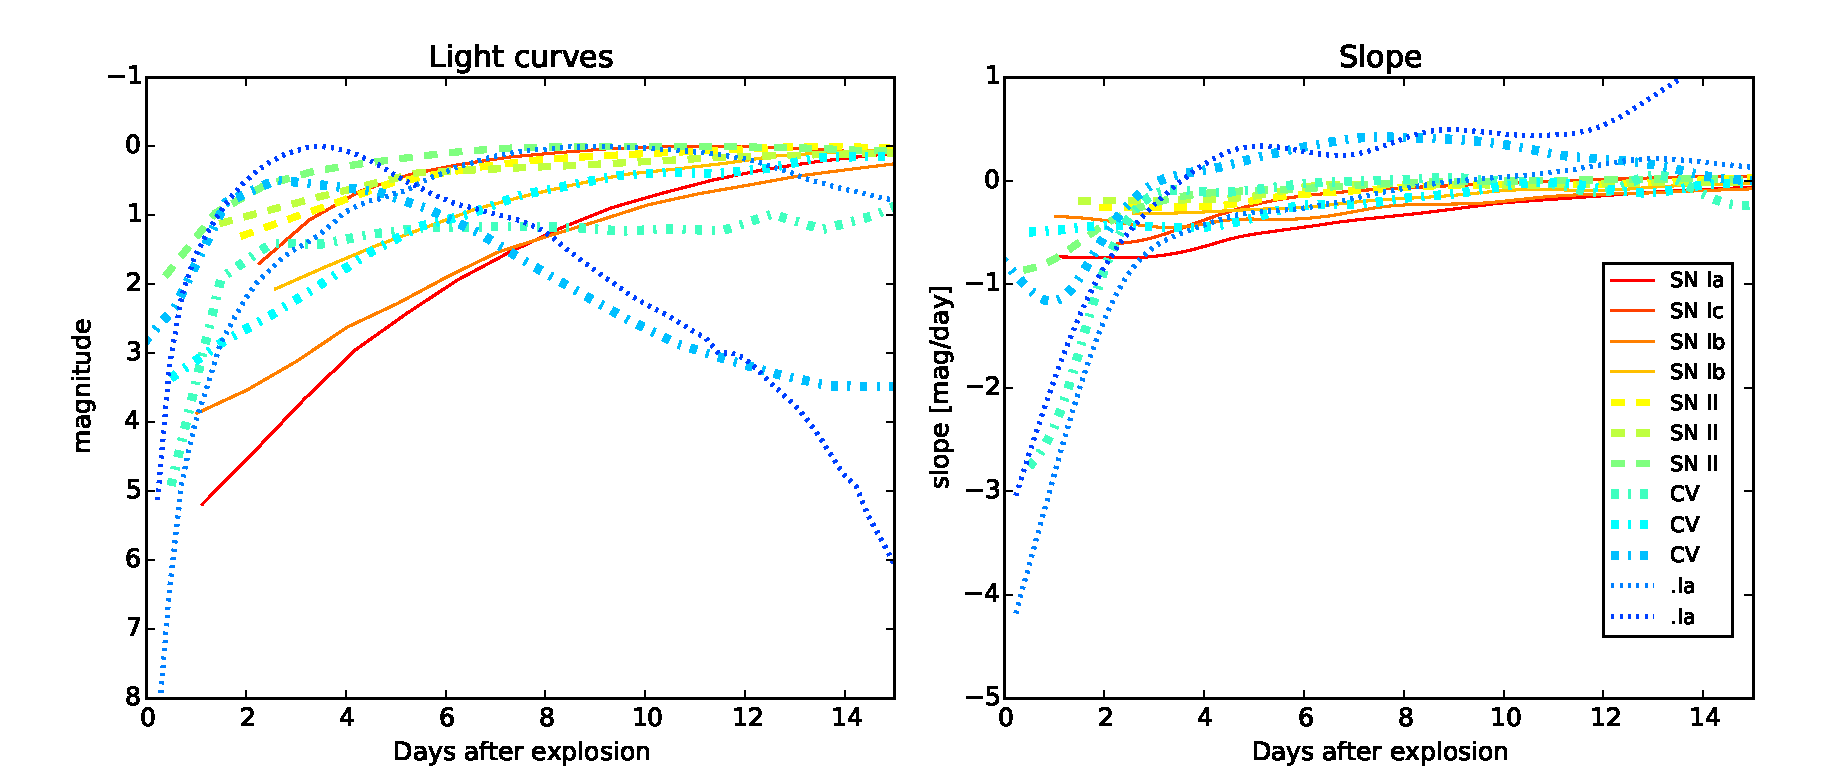
\includegraphics[width=0.6\textwidth]{figs/transients/earlyslope.pdf}
}
\caption{light curve slope [mag/days] of different type of transients as function of the phase from transient outburst/explosion.}
\label{fig:earlyslope}
\end{figure}

\begin{figure}[hbt]
\centerline{
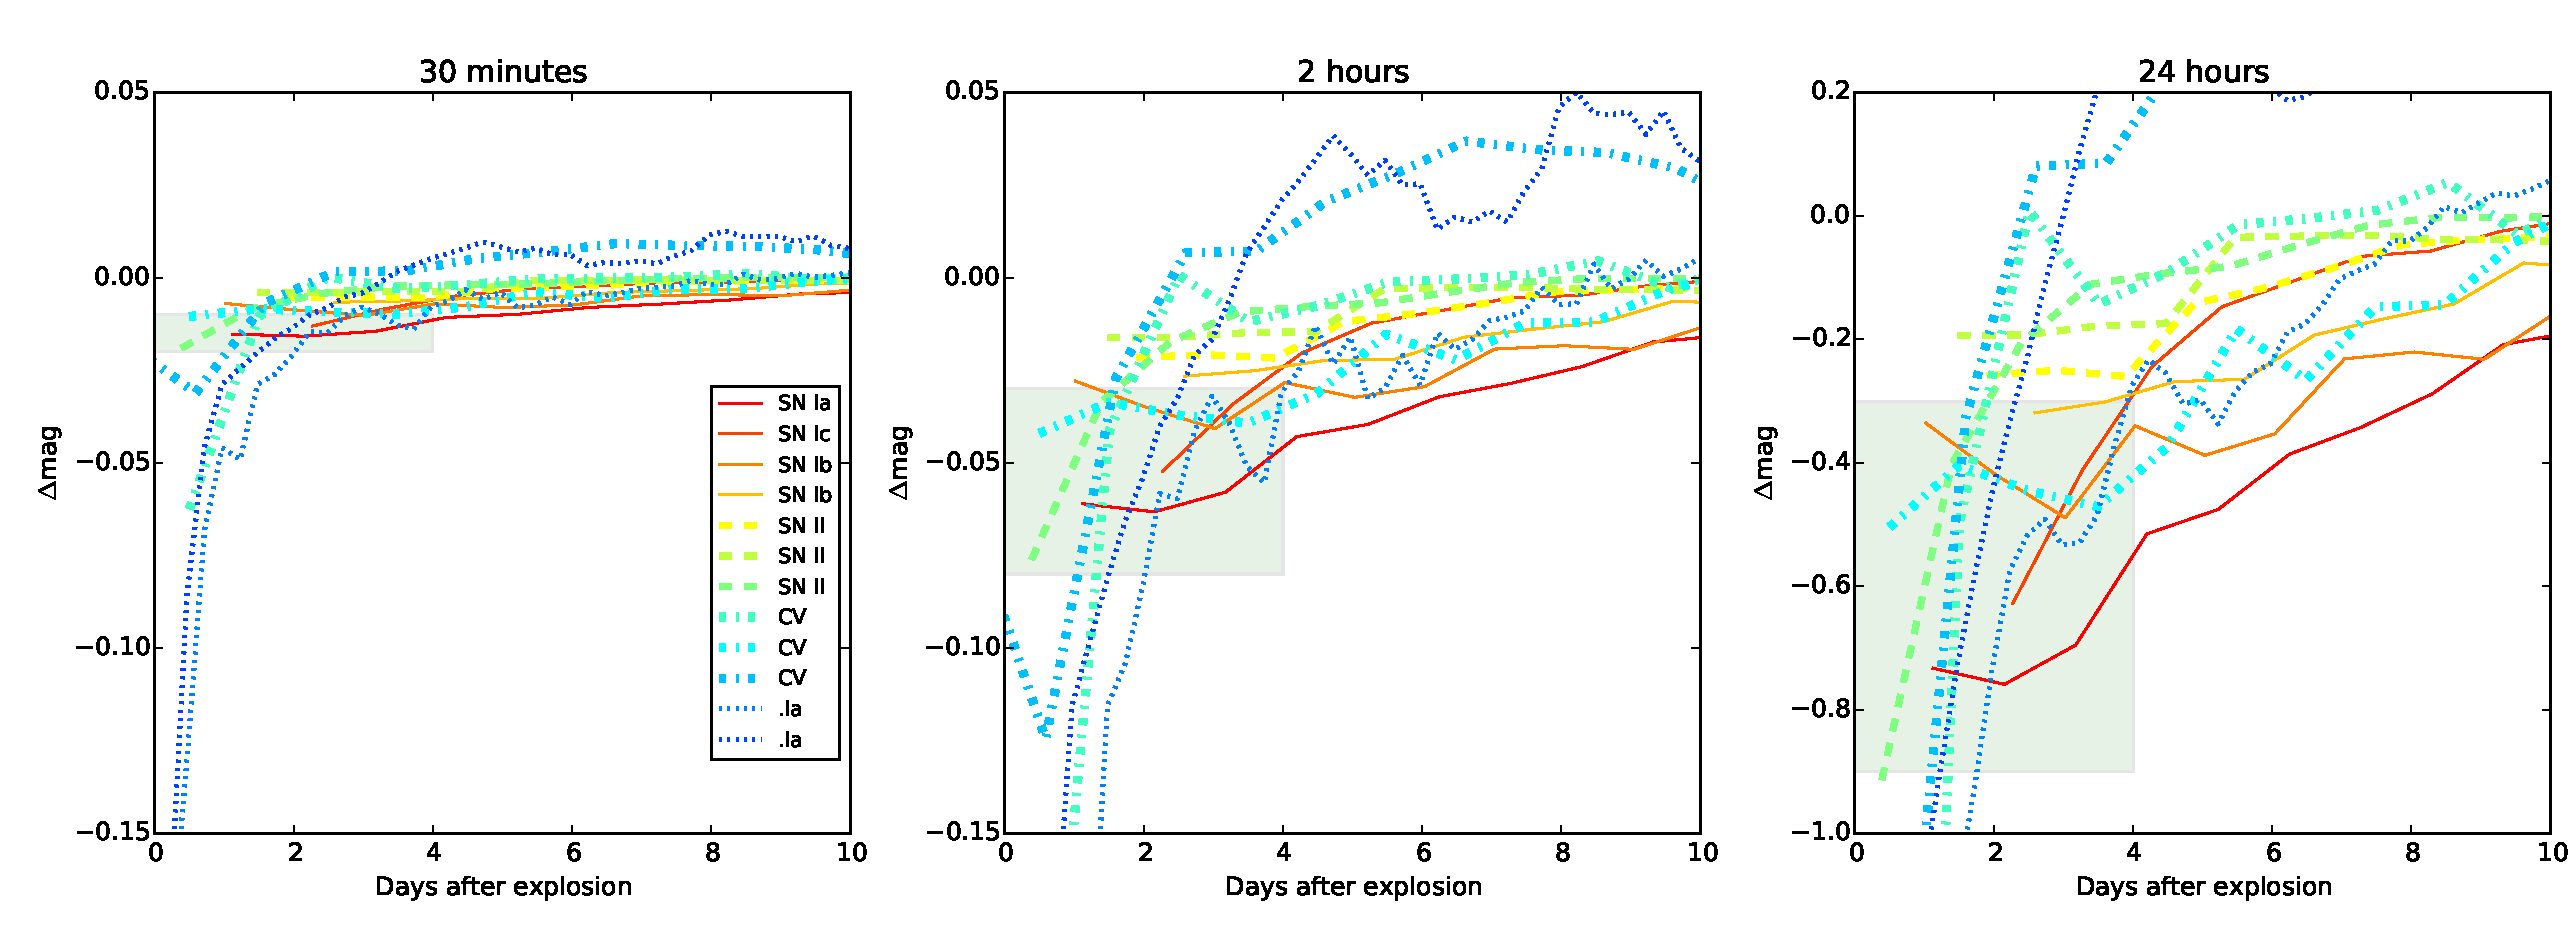
\includegraphics[width=0.6\textwidth]{figs/transients/earlyrise.pdf}
}
\caption{Expected difference magnitudes between two consecutive observations for a set of astronomical transients as a function of the phase of the transient. We consider the cases of the second observation occurring 30 minutes (left panel), 2 hours (central panel) and 24 hours (right panel) after the first observation. Data from: SN~Ia,  Olling et al 2015; SNII, Rubin et al 2016; SN~.Ia, 2010ApJ...715..767S; SN~Ib, Valenti et al 2011, Chao et al 2013; SN~Ic, Mazzali et al 2002; cv, Sokoloski et al. 2013, Finzell, et al in prep .
}
\label{fig:earlyrise}
\end{figure}
%%%%%%%%%%%%%%%%%%%%%%%%
%    Ineed to add the references
%
%Olling et al 2015, Nature, 521, 332O
%Rubin et al 2016, 2016ApJ, 820, 33R
%Valenti et al 2011, MNRAS, 416, 3138V
%Chao et al 2013,  ApJ, 775, 7C
%Mazzali et al, 2002, ApJ, 572L, 61M
%Sokoloski et al. 2013, 2013ApJ...770L..33S
%Finzell, et al in prep

